Tomando uma barra $AB$, homogênea e de seção transversal uniforme, apoiada em uma superfície lisa horizontal. Se for aumentada a temperatura da barra em um valor $\Delta T$, nota-se que ela se alonga de um valor $\delta_T$ que é proporcional tanto à variação de temperatura quanto ao comprimento da barra $L$. Tem-se, então:
\begin{equation}\label{eq:def-total}
	\delta_T=\alpha(\Delta T)L
\end{equation}

Onde $\alpha$ é a constante característica do material, chamada de \textit{coeficiente de dilatação térmica}. Como $L$ e $\delta_T$ são expressos em unidades de comprimento, $\alpha$ representa uma quantidade \textit{por grau C} ou \textit{por grau F}, dependendo de como a temperatura é expressada.

À deformação total $\delta_T$ está relacionada uma deformação específica $\varepsilon_T=\delta_T/L$. Reescrevendo a Equação~\eqref{eq:def-total}:
\begin{equation}
	\varepsilon_T=\alpha(\Delta T)
\end{equation}

Onde $\varepsilon_T$ é chamada de \textit{deformação térmica específica}, uma vez que é causada por variação de temperatura na barra. No caso considerado não há tensões relacionadas com a deformação $\varepsilon_T$.

\begin{figure}[H]
	\begin{center}
	\caption{Aumento de comprimento devido o acréscimo de temperatura.}
    	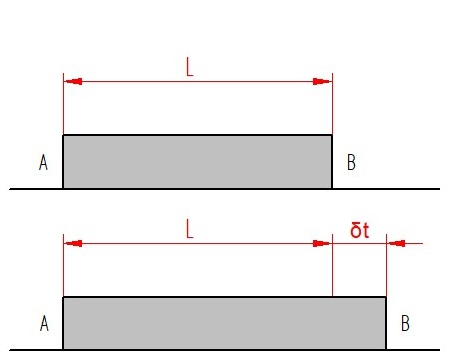
\includegraphics[width=0.5\textwidth]{Resistencia-dos-materiais/Imagens/Variacao-de-temperatura.jpg}
	\end{center}
\end{figure}

Agora, um caso específico. Considerando uma barra $AB$ de comprimento $L$, colocada entre dois anteparos fixos, separados por uma distância $L$. Elevando-se $\Delta T$, o alongamento da barra é nulo, pois os anteparos impedem qualquer deformação. Sendo a barra homogênea e de seção uniforme, a deformação específica em qualquer ponto é $\varepsilon=\delta_t/L$, também nula. Entretanto, para evitar o alongamento da barra, os anteparos vão aplicar sobre ela as forças $P$ e $P'$ após a elevação da temperatura. É criado um estado de tensão na barra (sem que ocorram deformações específicas).

\begin{figure}[H]
	\begin{center}
	\caption{Aumento de temperatura sem deformação.}
    	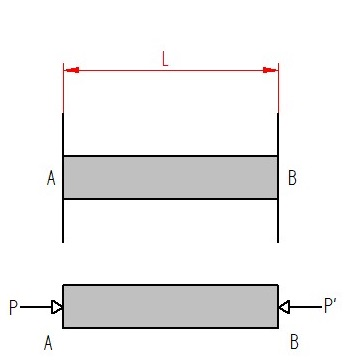
\includegraphics[width=0.5\textwidth]{Resistencia-dos-materiais/Imagens/Variacao-de-temperatura-sem-deformacao.jpg}
	\end{center}
\end{figure}